\section{Appendix Roadmap}

The appendix is intentionally skeletal until the protocol is fixed. Complete the subsections below without moving secondary detail back into the eight page main paper.

\section{Full Study Protocol}

\subsection{Corpus provenance, preprocessing, and leakage controls}
\label{sec:corpora_controls}
The project documents five candidate corpus lanes. Dreaddit's official train
partition is provisionally assigned to development, its official test partition
to a secondary in-domain audit, and all 11 CaCHe focus groups to the
held-out cross-domain confirmatory evaluation. KODIS is prepared only for a
private, unsplit exploratory role. CaSiNo and the AMI scenario-meeting subset
remain source-inventory dialogue candidates. KODIS, CaSiNo, and AMI have no
frozen manuscript experiment role, approved model or rater pathway, completed
contextual privacy review, or sampling eligibility.

Dreaddit is a publicly downloadable English Reddit corpus for stress detection. Its released labeled subset contains 3,553 human annotated segments from 2,929 posts across ten subreddits in five domains \citep{turcan2019dreaddit}. The archive provides official train and test partitions and post identifiers, but no author identifier. It therefore supports segment to post provenance and document concentration checks, not participant counts or participant level claims. The author archive contains 2,838 train segments from 2,343 posts and 715 test segments from 586 posts. It contains no README or dataset license. We retain text, the stress label, subreddit, and sentence range in the restricted analysis copy. We omit original post identifiers, timestamps, engagement measures, the internally inconsistent confidence field, and unused lexical features. Project specific identifiers preserve post grouping without exposing the released post identifier. The official splits have no post identifier overlap, but three exact texts occur in both partitions under different identifiers and conflicting labels. We retain those rows for audit but make the three training copies and 18 later within train exact duplicates ineligible for sampling, leaving 2,817 development segments and 715 audit segments before privacy quarantine. A checked exact-date rule then quarantines 13 complete development post clusters and three audit clusters, leaving 2,804 development and 712 audit candidate segments, or 3,516 segments and 301,279 whitespace delimited words in total. The remaining text still requires contextual privacy review.

The CaCHe deposit contains 11 participant-numbered and selectively redacted focus-group transcripts about how COVID-19 affected schooling, sexual behaviour, and sexual and reproductive health in western Kenya \citep{mehta2024cache2}. The source study reports six groups with 54 adolescent girls and young women and five with 53 community men. Sessions used English, Swahili, Dholuo, or a mixture and were translated into English \citep{awiti2024agyw}. The deposit is version 1, DOI \texttt{10.25417/uic.26495884.v1}, and CC BY 4.0. A fixed checksum allowlist verifies all 11 source files. Processing retains 3,575 participant turns and 369 collective turns; 3,076 participant turns meet the earlier three-word eligibility rule, but short and collective turns are no longer deleted and remain available as context. Each record has a stable focus-group and turn identifier, a transcript-local speaker identifier, source line spans, source hashes, translation status, the preceding moderator question, and prior-turn references. Normalization yields 106 observed transcript-local participant keys, one fewer than the 107 participants reported by the source paper; we do not claim complete participant coverage until this is reconciled. Conflicting source dates are recorded but excluded from model and router features.

The received KODIS workbook contains 2,860 unique dyads and 107 columns
\citep{hale2025kodis}. Its 2,085 human--human rows include 2,076 nonempty
dialogues with 27,121 parsed messages and 568,333 words; the remaining nine
have no transcript. Across all human--human rows, 1,712 are marked Resolution
and 373 Impass; among retained transcripts the counts are 1,708 and 368. The
median nonempty dialogue has 12 messages (interquartile
range 11--14) and 242 words (interquartile range 180--334). The private
exploratory builder excludes all 775 human--AI rows and all workbook surveys,
demographics, country, preferences, tactics, point totals, raw dyad identifiers,
and timestamps. It preserves nine seller-first dialogues and 271 dialogues with
at least one consecutive same-role transition rather than imposing artificial
alternation. All retained records have the single role
\texttt{exploratory\_unsplit}; the release has no stable cross-dialogue
participant identifier, so it cannot support participant-disjoint splitting or
participant-level denominators. This exploratory conversion is not a frozen
manuscript experiment or a substitute for contextual privacy review.

The acquired CaSiNo source is the official CC BY 4.0 repository snapshot
pinned to commit \texttt{2f6ed4a}. It contains 1,030 dyadic campsite
negotiation dialogues, 11,919 ordinary messages, 2,378 structured negotiation
events, and 228,675 whitespace delimited words in the ordinary messages
\citep{chawla2021casino}. The source paper reports 846 participants, but the
public JSON provides only two dialogue local role tokens and no stable
cross-dialogue participant token. We therefore reject the supplied 900/30/100
random split for WarrantRoute, do not reconstruct linkage from participant
profiles or text, and leave the corpus unassigned unless trustworthy provider
linkage becomes available or the entire corpus is preregistered in one unsplit
role after the governance gates are satisfied. Any adopted CaSiNo adapter must
retain ordinary dialogue text and turn lineage only and exclude structured
events, annotations, demographics, personality measures, preferences, free-text
reasons, negotiation outcomes, and raw identifiers.

The acquired AMI manual annotation artifact contains a selectively extracted
source inventory for 138 elicited scenario meetings in 35 meeting series. The
four person meetings are English product design discussions. The selected
files contain 793,764 transcribed words, 69,258 speech segment
elements, and mappings for 140 global source speaker identifiers. These form
35 meeting and speaker connected components, 33 with four meetings and two
with three meetings \citep{carletta2006ami}. No audio, video, signals, slides,
questionnaires, demographics, participant file, or nontranscript annotation
category was extracted. The official filename labels the manual annotations
as version 1.6.2, while the embedded README says release 1.7; we bind the
source by its exact URL, filename, size, and checksum rather than asserting
that those labels are equivalent. The corpus is not sampling eligible. A
adopted AMI transcript adapter must discard timing and raw source identifiers, and
all 35 meeting and speaker components must remain indivisible in any adopted
split.

\begin{table*}[t]
\centering
\scriptsize
\setlength{\tabcolsep}{2pt}
\renewcommand{\arraystretch}{0.92}
\begin{tabularx}{\textwidth}{@{}l>{\raggedright\arraybackslash}Xl>{\raggedright\arraybackslash}X@{}}
\toprule
Dataset & Context & Language & Inventory \\
\midrule
Dreaddit \citep{turcan2019dreaddit} & Social-media stress posts & English & \shortstack[l]{2,929 posts; 3,553 segments;\\3,516 candidate; 301,279 words} \\
CaCHe \citep{mehta2024cache2} & Sexual and reproductive health focus groups & Translated English & \shortstack[l]{11 groups; 3,944 turns;\\3,076 eligible; 98,735 words} \\
KODIS \citep{hale2025kodis} & Customer-service dispute dialogues & English & \shortstack[l]{2,085 human--human dyads;\\2,076 dialogues; 27,121 messages;\\568,333 words} \\
CaSiNo \citep{chawla2021casino} & Campsite negotiation dialogues & English & \shortstack[l]{1,030 dialogues; 11,919 messages;\\228,675 words} \\
AMI scenario \citep{carletta2006ami} & Product-design meetings & Spoken English & \shortstack[l]{138 meetings; 69,258 segments;\\793,764 words} \\
\bottomrule
\end{tabularx}
\caption{Corpus inventories. Dreaddit and CaCHe alone have provisional experimental roles; their counts are preparation inventories, not privacy-cleared samples or experimental outcomes. KODIS, CaSiNo, and AMI are internal candidate inventories and are not sampling eligible.}
\label{tab:dataset_statistics}
\end{table*}

For Table~\ref{tab:dataset_statistics}, a source is one Reddit post, focus
group, KODIS human--human dyad, CaSiNo dialogue, or AMI meeting. Dreaddit source
units are released labeled segments, and its candidate units exclude duplicate
texts and complete exact-date post clusters. CaCHe retained units
include participant and collective turns, while its eligible count applies the
earlier three word participant-turn rule. KODIS units are parsed role messages
from nonempty human--human transcripts. CaSiNo units are ordinary source
messages and exclude structured events. AMI units are upstream speech segment
elements. KODIS, CaSiNo, and AMI counts are not sampling eligible or common
analysis denominators.

Under this protocol, Dreaddit's official train partition is the sole development corpus for prompts, packet rules, controlled variants, routing features, and thresholds. Once those choices are frozen, its official test partition serves as the in-domain audit, and all 11 CaCHe focus groups serve as the held-out cross-domain evaluation. ``Held out'' refers to the experimental procedure, not model-training provenance. Because the deposit is public and its published themes are known, we do not describe it as unopened or model-unseen or use the published themes as scoring gold.

The power analysis and primary serious-error outcomes determine a common number of base
packets for the Dreaddit audit and CaCHe evaluation. Human review time is a
secondary implementation measure and matched-time comparison control. Sampling preserves post
clusters in Dreaddit and focus group and transcript local speaker clusters in
CaCHe. Both corpora use identical packet and context limits. Dreaddit labels
and published CaCHe themes may stratify audits but are not treated as thematic
ground truth or router features. KODIS, CaSiNo, and AMI enter no manuscript
generation, sampling,
or model selection procedure unless separately preregistered after corpus
specific validation and governance approval.

Packet generation has not begun and remains blocked until the governance gates are complete. After authorization, packet generation uses \fillin{CANDIDATE-GENERATION MODEL SNAPSHOTS} and \fillin{GENERATION PROCEDURE}. The protocol requires retention of prompts, decoding settings, context order, run identifiers, source spans, and human revisions and prohibits selection of test outputs after inspection of their quality. Candidate-generation models and LLM reviewers require separate actor identifiers, authorization records, prompts, and run manifests. Only text or transcripts covered by the documented governance arrangement are eligible for processing, and protected material cannot be sent to an external model unless the access terms and our institution permit it. Public release is limited to aggregate outputs, schemas, and text specifically cleared for release.

\fillin{CURRENT INSTITUTIONAL DETERMINATION; SOURCE, PLATFORM, CANDIDATE-GENERATION, LLM-REVIEWER, AND HUMAN-RATER AUTHORIZATIONS FOR DREADDIT, CaCHe, KODIS, CASINO, AND AMI; KODIS AND CASINO UNSPLIT ROLE DECISIONS; AMI COMPONENT SPLIT; RATER EXCERPT RULES; FINAL PACKET COUNTS; ACTOR REGISTRY; MODEL SNAPSHOTS; PROMPTS; DECODING SETTINGS; RUN COUNTS; AND FROZEN MANIFEST HASHES}.

\subsection{Role definitions and recruitment}
\label{sec:reviewer_protocol}
\fillin{ELIGIBILITY FOR RESEARCHERS WITHOUT SPECIALIST EXPERTISE, QUALITATIVE METHODS EXPERTS, AND DOMAIN EXPERTS; HANDLING OF DUAL EXPERTISE; RECRUITMENT; COMPENSATION; POSITIONALITY; EXCLUSIONS; AND INDEPENDENCE SAFEGUARDS}. For RQ2, \fillin{LLM REVIEWER SNAPSHOTS, GENERALIST/METHODS/DOMAIN ROLE PROMPTS, RESPONSE SCHEMA, ONE-PACKET CONTEXT RULE, REPETITIONS, AGGREGATION, RETRIES, TERMINAL-FAILURE HANDLING, PRE-HUMAN OUTPUT-SEAL HASH, AND THE RULE FOR SELECTING ROLE OUTPUTS}.

\subsection{Complete annotation instrument}
The three packet-level rating prompts are: (1) \emph{How fully does the cited evidence support the core interpretive meaning in context?} (evidential credibility); (2) \emph{How well does the packet preserve consequential differences, dissent, counterevidence, less-frequent or boundary cases, and contextual qualifications?} (voice-and-boundary preservation); and (3) \emph{How well do the strength and breadth of the claim, including causal or group-level language, match the supplied evidence?} (scope calibration).

For each question, 1 means not adequate, 2 major problems, 3 partially adequate and requiring material revision, 4 mostly adequate with only minor issues, and 5 fully adequate. The tutorial specification requires construct-specific examples at each anchor. For rating $r_{ijm}$ from rater $i$ on packet $j$, the analysis specification retains the full ordinal response; the descriptive adequacy rate for measure $m$ is the proportion of evaluable rater--packet judgments scored 4 or 5:
\begin{description}
    \item[Evidential credibility.] A 1 indicates absent, unverifiable, misattributed, or contradictory evidence; a 3 indicates that the core meaning is partly supported but a material link or qualifier lacks evidence; and a 5 indicates that every material part of the core interpretation is directly warranted by sufficient contextual evidence.
    \item[Voice-and-boundary preservation.] A 1 indicates that a consequential voice, counterexample, or contextual distinction is erased or reversed; a 3 retains the main pattern but underplays a meaningful viewpoint or boundary; and a 5 retains all consequential variation, dissent, less-frequent cases, and contextual qualifications visible in the packet.
    \item[Scope calibration.] A 1 indicates that claim breadth, polarity, or causal strength is incompatible with the evidence; a 3 has the broadly appropriate direction but requires a material change in scope or strength; and a 5 fully matches participant-, group-, and corpus-level scope and makes no stronger causal or prevalence claim than the evidence permits.
\end{description}
Scores 2 and 4 represent the corresponding intermediate judgments under the common anchors. Raters select ``cannot judge'' when the supplied excerpts, local context, or source-coverage summary are insufficient for the specified dimension.
\begin{equation}
A_m =
\frac{\sum_{i,j}\mathbb{1}\!\left(r_{ijm}\in\{4,5\}\right)}
     {\sum_{i,j}\mathbb{1}\!\left(r_{ijm}\text{ is evaluable}\right)}.
\end{equation}
``Cannot judge'' is neither a midpoint nor a failure and is reported with its own denominator. Confidence has separate anchors from 1 (very uncertain) to 5 (very certain). Exact-string and source-offset checks are recorded as deterministic diagnostics; raters judge whether verified excerpts warrant the interpretation in context.

\fillin{CONSENT TEXT, TUTORIAL EXAMPLES, COMPREHENSION CHECKS, ACCEPT/REVISE/REJECT/ESCALATE WORDING, HUMAN CANNOT-JUDGE RULE, LLM ABSTENTION AND FAILURE RULES, SHARED RESPONSE CONTRACT, RATIONALE PROMPT, AND TIMING DISCLOSURE}.

\subsection{Artifact-quality definitions and matching}
\label{sec:artifact_metrics}

Plural-reference coverage is calculated only for complete, natural-output code and theme inventories, not from sampled packets or controlled twins. The protocol requires multiple analysts to produce code and theme concepts independently and requires the pooled reference space to be frozen before test-output inspection, after merging only concepts adjudicated to be equivalent and retaining the originating analyst and source provenance. The resulting pool is interpreted as a bounded set of defensible concepts available to the study team, not universal thematic ground truth.

For output level $\ell\in\{\text{code},\text{theme}\}$, let $P_\ell$ be the frozen pooled concepts and $G_\ell$ the generated concepts. Independent experts blinded to system condition may make many-to-many conceptual matches, denoted by $p\sim g$. Coverage is
\begin{equation}
C_\ell =
\frac{\left|\left\{p\in P_\ell:\exists g\in G_\ell,\;p\sim g\right\}\right|}
     {|P_\ell|}.
\end{equation}
The reporting contract requires separate code and theme coverage with preregistered uncertainty intervals, a list of unmatched reference concepts, retained matching disagreements, and separate evidential review before any unmatched generated concept is counted as an error. It also requires generated code and theme counts, unmatched generated concepts, split and merge patterns, redundancy, and the human-audited unsupported-concept rate. The router cannot access this measure because it relies on the analyst reference space. The three ordinal measures and plural-reference coverage remain separate; no omnibus quality score is permitted.

For controlled variants, the primary manipulation check maps unsupported evidence to evidential credibility; source concentration, counterevidence loss, and contextual flattening to voice-and-boundary preservation; and unsupported abstraction to scope calibration. The analysis also reports cross-construct effects rather than assuming that each defect affects only one measure. Plural-reference coverage is restricted to natural-output inventories and does not serve as a manipulation check for controlled twins.

\subsection{Packet construction and assignment}
\fillin{NATURAL ITEM SAMPLING, CONSTRUCTION OF CONTROLLED VARIANTS, VETTING, MANIPULATION CHECKS, RANDOMIZATION, INCOMPLETE BLOCK ASSIGNMENT, AND BLINDING}.

\subsection{Power and confirmatory analysis}
\fillin{PILOT VARIANCE COMPONENTS, SIMULATION DESIGN, POWER TARGET, RQ1 PRIMARY CONTRASTS, RQ2 PAIRED HUMAN--LLM CONTRASTS, MODEL EQUATIONS, MULTIPLICITY PLAN, FALLBACKS, AND EXCLUSIONS}.

\subsection{Routing implementation}
\fillin{RQ1 AND RQ2 FEATURE DEFINITIONS, HUMAN- AND LLM-GENERALIST INPUT MAPPING, PREPROCESSING, ROUTING MODEL, HYPERPARAMETERS, FALSE-ACCEPTANCE CEILING, THRESHOLDS, MATCHED-HUMAN-TIME SENSITIVITY, CROSS FITTING, FREEZE DATE, AND TEST ACCESS LOG}.

\section{Detailed Ethics and Data Governance}
\label{sec:detailed_ethics}

\subsection{Source review and access conditions}

Approval of an original collection does not authorize this secondary study, model processing, or disclosure to raters. Real-text processing and rater disclosure remain blocked until the record contains our institution's determination, its scope and date, and the governing source, platform, and access terms for each corpus.

The received KODIS README records collection dates, field definitions, and a
required scholarly citation, but it does not state a data license, secondary-use
consent, or authorization for external model processing or rater disclosure.
We therefore keep the exploratory output local and do not treat receipt of the
workbook as permission for a manuscript experiment \citep{hale2025kodis}.

The CaCHe source study reports written consent and review by Rush University Medical Center (22011311), Maseno University Ethics Review Committee (MSU/DRPI/MUERC/01021/21), and University of Illinois Chicago (2022-0220), with a favorable opinion from Liverpool School of Tropical Medicine (21-087) \citep{awiti2024agyw}. The CaSiNo paper reports institutional review, informed consent covering collection and later use, a right to withdraw, and removal of MTurk and HIT identifiers before public release \citep{chawla2021casino}. Although that paper calls the released data anonymized, we do not adopt that label: dialogue and rich participant metadata can remain identifying. The AMI site documents European Commission ethics review and signed consent that anticipated possible release to the wider research community; its consent form states that anonymity could not be guaranteed and allowed participants to request removal \citep{amietics}. The CC BY 4.0 licenses for CaSiNo and AMI do not grant privacy or personality rights or authorize this project's model processing, rater disclosure, retention, or release. We did not find an ethics determination, Reddit author consent, privacy procedure, or dataset license in the Dreaddit paper or author archive \citep{turcan2019dreaddit}; any use therefore remains conditional on a documented institutional and platform basis.

\subsection{Project safeguards and rater protections}

We do not describe the corpora as anonymous. Dreaddit retains searchable verbatim posts. CaCHe contains sensitive sexual and reproductive health narratives that may remain identifying despite participant numbers and selective redaction. KODIS combines role-play dialogue with country, survey, preference, tactics, and outcome fields; the private exploratory output retains only dialogue text, minimal row lineage, role, and aggregate diagnostics. CaSiNo raw records combine dialogue with demographics, personality measures, preferences, free text reasons, and outcome surveys; those metadata remain excluded from any authorized working output. AMI source XML contains transcript text, precise timing, and attribute bearing source identifiers; any authorized working output must omit timings and raw identifiers. Restricted analysis copies use project pseudonymous identifiers, minimize fields, mask direct identifier patterns, and preserve protected linkage information separately. Pattern masking does not replace contextual privacy review. Protected text is not sent to a model or service unless its processing, retention, and training terms are approved. \fillin{STATE STORAGE LOCATION, ACCESS ROLES, RETENTION PERIOD, DELETION PROCEDURE, APPROVED MODEL PROVIDERS, AND PROVIDER RETENTION OR TRAINING SETTINGS}.

No excerpt may be shown to raters or considered for release unless it passes a two-person privacy and permissions review. Public artifacts are limited to aggregate results, code, prompts, schemas, and only text or ratings specifically cleared for release. Raw hashes of short sensitive excerpts are not published without an assessment of linkage risk. Enrollment requires a study-specific consent form and privacy warning; raters may withdraw under the approved procedure and participate voluntarily outside supervisory, employment, grading, or authorship decisions. The storage policy requires identifiers to remain separate from responses. \fillin{STATE RECRUITMENT CHANNELS, ELIGIBILITY, COMPENSATION AND RATE JUSTIFICATION, WITHDRAWAL HANDLING, RATER DEMOGRAPHICS, AND FINAL CONSENT LANGUAGE}. Routing is a research review aid, not a clinical or participant-level decision system; random audits and false-acceptance reporting address, but do not remove, the risk of false reassurance.

\section{Supplementary Results}
\label{sec:appendix_results}

The source-grounded artifact profile below is now part of the compiled results
shell. Its cells remain blank because corpus inventories cannot substitute for
human ordinal ratings, reference-concept matching, or serious-error judgments.
No result rows are assigned to KODIS, CaSiNo, or AMI unless a separate
preregistration assigns an experimental role.

\begin{table*}[t]
\centering
\scriptsize
\setlength{\tabcolsep}{2.1pt}
\begin{tabularx}{\textwidth}{@{}>{\raggedright\arraybackslash}X>{\raggedright\arraybackslash}Xrrrrrrrrrr@{}}
\toprule
\shortstack[l]{Corpus /\\evaluation role} & System & \shortstack{Complete\\inventories} & \shortstack{Rated\\packets} & \shortstack{Integrity\\pass $n/N$} & \shortstack{Evidential\\adequacy} & \shortstack{Voice/boundary\\adequacy} & \shortstack{Scope\\adequacy} & \shortstack{Code\\coverage} & \shortstack{Theme\\coverage} & \shortstack{Cannot\\judge} & \shortstack{Serious\\error} \\
\midrule
CaCHe / cross-domain confirmatory & Frozen primary & \blankcell & \blankcell & \blankwide & \blankwide & \blankwide & \blankwide & \blankwide & \blankwide & \blankwide & \blankwide \\
CaCHe / cross-domain confirmatory & Frozen comparator & \blankcell & \blankcell & \blankwide & \blankwide & \blankwide & \blankwide & \blankwide & \blankwide & \blankwide & \blankwide \\
Dreaddit / in-domain audit & Frozen primary & \blankcell & \blankcell & \blankwide & \blankwide & \blankwide & \blankwide & \blankwide & \blankwide & \blankwide & \blankwide \\
Dreaddit / development & Selected primary & \blankcell & \blankcell & \blankwide & \blankwide & \blankwide & \blankwide & \blankwide & \blankwide & \blankwide & \blankwide \\
\bottomrule
\end{tabularx}
\caption{Source-grounded artifact profile. Adequacy is the percentage of evaluable packet ratings scored 4 or 5; ``cannot judge'' has a separate denominator. Plural-reference coverage is computed separately for complete code and theme inventories. Integrity requires schema and assignment completeness, quotation/source fidelity, valid provenance edges, and cross-source support for cross-source themes. Report 95\% intervals clustered by the preregistered sampling unit.}
\label{tab:artifact_quality_profile}
\end{table*}


\begin{table*}[h]
\centering
\small
\setlength{\tabcolsep}{4pt}
\begin{tabular}{lccccc}
\toprule
Evaluator group and construct & \shortstack{Krippendorff\\$\alpha$} & Gwet AC2 & Raw agreement & Cannot judge & Median time \\
\midrule
Researchers: credibility & \blankcell & \blankcell & \blankcell & \blankcell & \blankcell \\
Researchers: voice/boundary & \blankcell & \blankcell & \blankcell & \blankcell & \blankcell \\
Researchers: scope calibration & \blankcell & \blankcell & \blankcell & \blankcell & \blankcell \\
Methods experts: credibility & \blankcell & \blankcell & \blankcell & \blankcell & \blankcell \\
Methods experts: voice/boundary & \blankcell & \blankcell & \blankcell & \blankcell & \blankcell \\
Methods experts: scope calibration & \blankcell & \blankcell & \blankcell & \blankcell & \blankcell \\
Domain experts: credibility & \blankcell & \blankcell & \blankcell & \blankcell & \blankcell \\
Domain experts: voice/boundary & \blankcell & \blankcell & \blankcell & \blankcell & \blankcell \\
Domain experts: scope calibration & \blankcell & \blankcell & \blankcell & \blankcell & \blankcell \\
\bottomrule
\end{tabular}
\caption{Reliability shell for human ratings on the three ordinal artifact-quality measures. Report intervals and score prevalence in the final appendix; LLM repetition behavior, confidence, and routing-model calibration are reported separately.}
\label{tab:artifact_reliability}
\end{table*}

\begin{table*}[h]
\centering
\scriptsize
\setlength{\tabcolsep}{2.5pt}
\begin{tabular}{lccccc}
\toprule
\multicolumn{6}{c}{\textcolor{gray}{\textit{Placeholder only---no experimental results are available}}} \\
\addlinespace[2pt]
Policy & Expert minutes & Serious-error recall & False acceptance & Difference from both experts & Errors per expert hour \\
\midrule
Researchers only & 0 (design) & \fillin{EST. [CI]} & \fillin{EST. [CI]} & \fillin{$\Delta$ [CI]} & Not applicable \\
Random & \fillin{MIN.} & \fillin{EST. [CI]} & \fillin{EST. [CI]} & \fillin{$\Delta$ [CI]} & \fillin{EST.} \\
Uncertainty routing & \fillin{MIN.} & \fillin{EST. [CI]} & \fillin{EST. [CI]} & \fillin{$\Delta$ [CI]} & \fillin{EST.} \\
WarrantRoute & \fillin{MIN.} & \fillin{EST. [CI]} & \fillin{EST. [CI]} & \fillin{$\Delta$ [CI]} & \fillin{EST.} \\
Both expert groups & \fillin{MIN.} & \fillin{EST. [CI]} & \fillin{EST. [CI]} & Reference by design & \fillin{EST.} \\
\bottomrule
\end{tabular}
\caption{Secondary matched-human-time reporting shell for the RQ1 CaCHe routing comparison. No experimental results are reported. Populate estimates and intervals only from the frozen confirmatory analysis export. Zero specialist minutes for the researchers-only condition and the reference status of both-expert review are protocol design constants, not observed outcomes.}
\label{tab:routing_policy_detail}
\end{table*}

\begin{table*}[h]
\centering
\small
\setlength{\tabcolsep}{4pt}
\begin{tabular}{lccccc}
\toprule
Routing configuration & Dreaddit dev. & Dreaddit audit & CaCHe & Recall change & Review minutes \\
\midrule
Full features & \blankcell & \blankcell & \blankcell & \blankcell & \blankcell \\
No disagreement & \blankcell & \blankcell & \blankcell & \blankcell & \blankcell \\
No abstention & \blankcell & \blankcell & \blankcell & \blankcell & \blankcell \\
No provenance & \blankcell & \blankcell & \blankcell & \blankcell & \blankcell \\
Confidence only & \blankcell & \blankcell & \blankcell & \blankcell & \blankcell \\
\bottomrule
\end{tabular}
\caption{Secondary corpus and routing-feature sensitivity shell. Define the reported metric in the final caption; no experimental results are reported.}
\label{tab:transfer_ablation}
\end{table*}

\begin{figure*}[h]
\centering
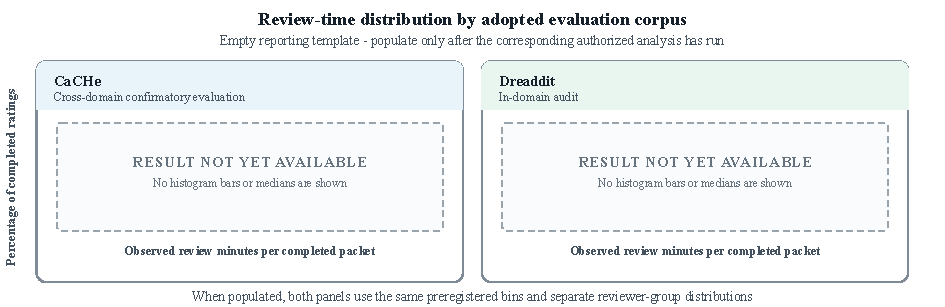
\includegraphics[width=\textwidth]{figures/review_time_histogram_shell.pdf}
\caption{Secondary histogram reporting template for observed human review time per completed packet by reviewer group and adopted corpus. Review time is not a research question, and no experimental results are reported. When populated from the frozen RQ1 export, both panels use the same preregistered bins and show the percentage of completed ratings; median lines are derived from those observations. LLM latency, tokens, and cost are reported separately.}
\label{fig:review_time_distribution}
\end{figure*}

\fillin{ADD ROUTE-TO-USEFUL-ROLE CONFUSION MATRICES, SELECTIVE-RISK VERSUS REVIEW-COVERAGE CURVES, RESULTS BY FAILURE FAMILY, RQ2 LLM--HUMAN CONTRASTS WHEN AVAILABLE, LLM ABSTENTION AND TERMINAL-FAILURE COUNTS, COMPARISONS OF NATURAL AND CONTROLLED ITEMS, CONFIDENCE AND ROUTING-MODEL CALIBRATION PLOTS, RATIONALE ANALYSIS, AND ROBUSTNESS CHECKS}.

\section{Reproducibility and Governance Checklist}

\begin{itemize}
    \item[$\square$] Confirm institutional, source or platform, model processing, and rater access conditions for Dreaddit, CaCHe, KODIS, CaSiNo, and AMI; confirm unsplit roles for KODIS and CaSiNo if adopted; validate AMI transcript preprocessing and freeze component isolated splits; then freeze the analytic contract, prompts, model snapshots, and manifests.
    \item[$\square$] Obtain ethics determination and finalize voluntary recruitment and withdrawal procedures that avoid coercion.
    \item[$\square$] Freeze human and LLM role criteria, item manifest, actor registry, LLM reviewer snapshots and prompts, the four metric definitions and anchors, plural-reference construction and matching rules, assignment, exclusions, and power analysis.
    \item[$\square$] Freeze routing features and thresholds, RQ1 and RQ2 primary outcomes, LLM repetitions and failure rules, the secondary matched-human-time analysis, and analysis code before candidate generation or LLM rating on CaCHe.
    \item[$\square$] Release only packets cleared by the two-person excerpt review, permitted ratings, prompts, code, model and run metadata, non-text manifest hashes, and text-derived hashes only when source terms permit and linkage-risk review clears them, plus a datasheet.
    \item[$\square$] Replace every \texttt{\textbackslash fillin}, \texttt{\textbackslash blankcell}, and \texttt{\textbackslash blankwide}; set \texttt{\textbackslash predatadraftfalse}; verify the eight page boundary; and update the abstract last.
\end{itemize}
